\section{Results}
\label{sec:results}

\begin{figure}[htbp!]
\begin{center}
    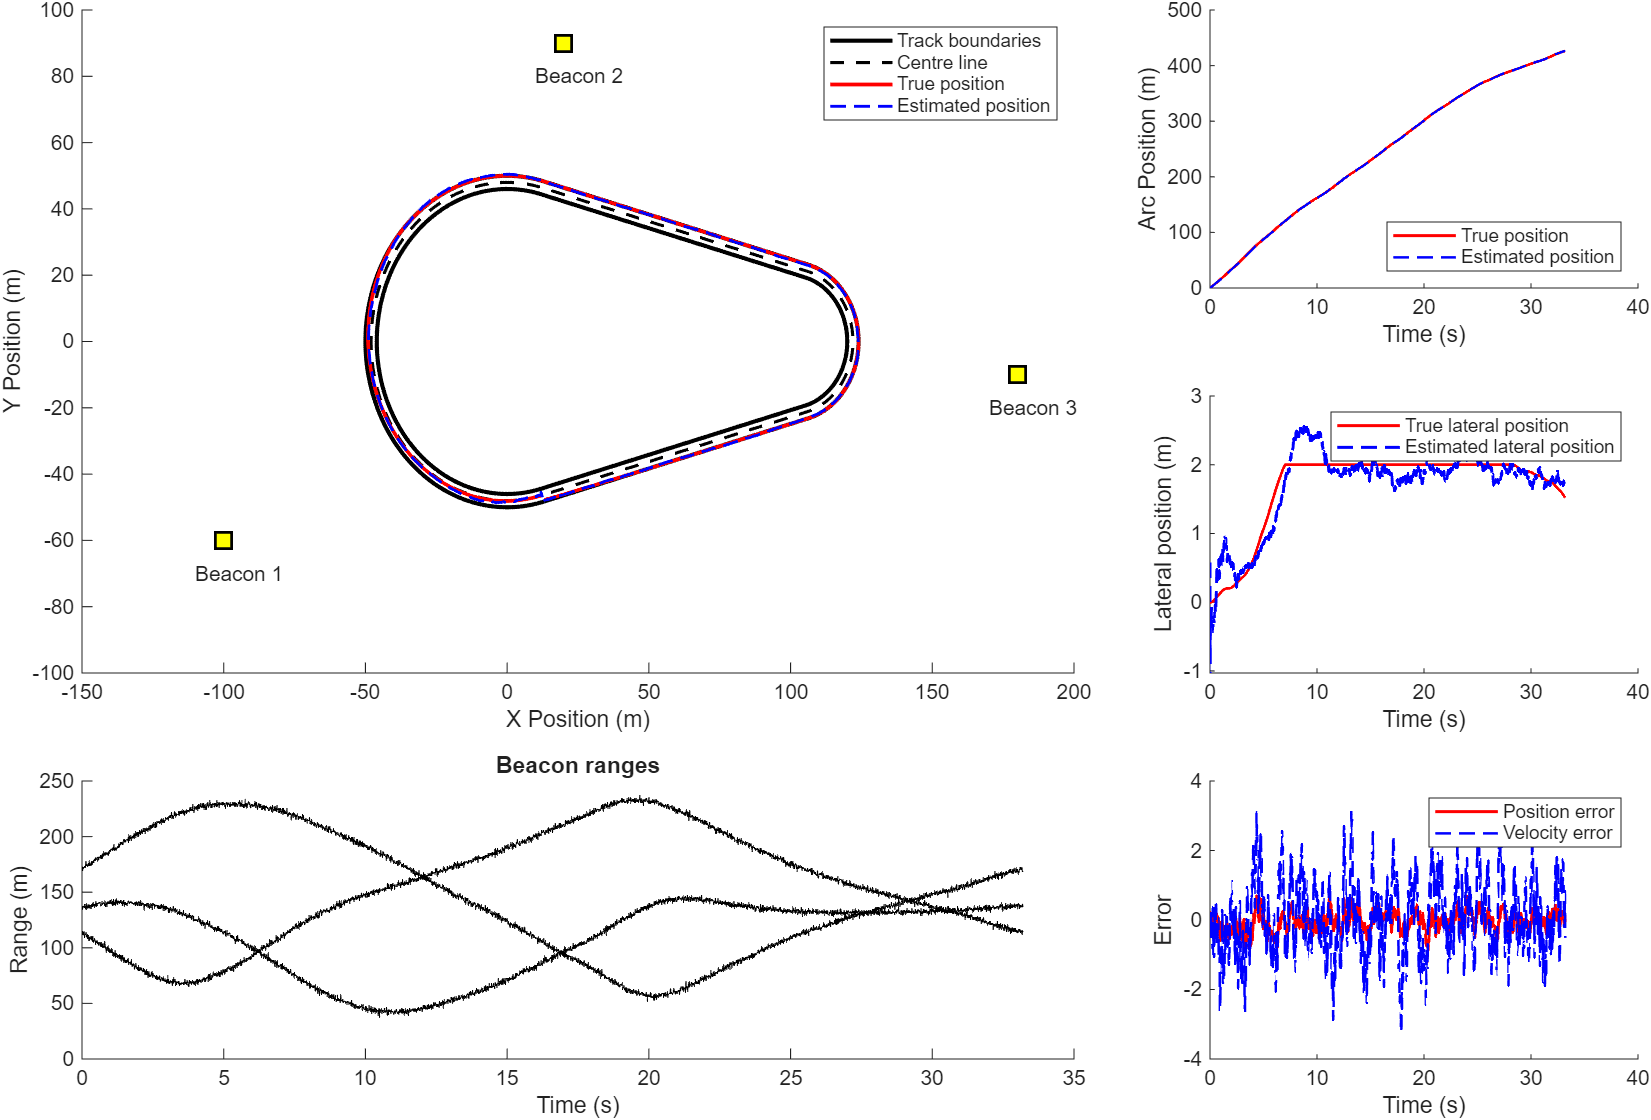
\includegraphics[scale=0.5]{figures/ekf-trajectories.png}
\end{center}
\caption{Simulation of the EKF on the track trajectory (top left), associated range from each beacon (bottom left), arc position trajectory, (top right), lateral position trajectory (middle right) and error between the true arc position and arc velocity (bottom right)}
\label{fig:ekf-trajectory}
\end{figure}

Figure~\ref{fig:ekf-trajectory} demonstrates the trajectory for one full lap of the track. It is obvious that the track dynamics are unphysical, as the lateral position of the vehicle "saturates" due to the accumulation of noise (lateral acceleration) in the system.

The estimator performs well with regards to arc position $s$, as the noise imposed on the beacon measurements is small relative to the total track trajectory (approx. 400m).
The does not perform as well for lateral position, given that the total domain over which the vehicle can move laterally (4m) is small relative to the noise imposed on the measurement model.

It should be noted that velocity is also estimated rather poorly, as the system must infer this from the position measurements.

\begin{figure}[htbp!]
\begin{center}
    \includegraphics[scale=0.5]{figures/monte-carlo.png}
\end{center}
\caption{Monte Carlo simulation for each state variable for $n=100$ runs}
\label{fig:monte-carlo}
\end{figure}

Figure~\ref{fig:monte-carlo} highlights the trajectories for 100 simulated trajectories of each state variable. It is obvious that the Gaussian noise model is not appropriate for a model requiring state constraints, as the bounds on the state dynamics effectively result in the vehicle travelling along the wall.

\begin{figure}[htbp!]
\begin{center}
    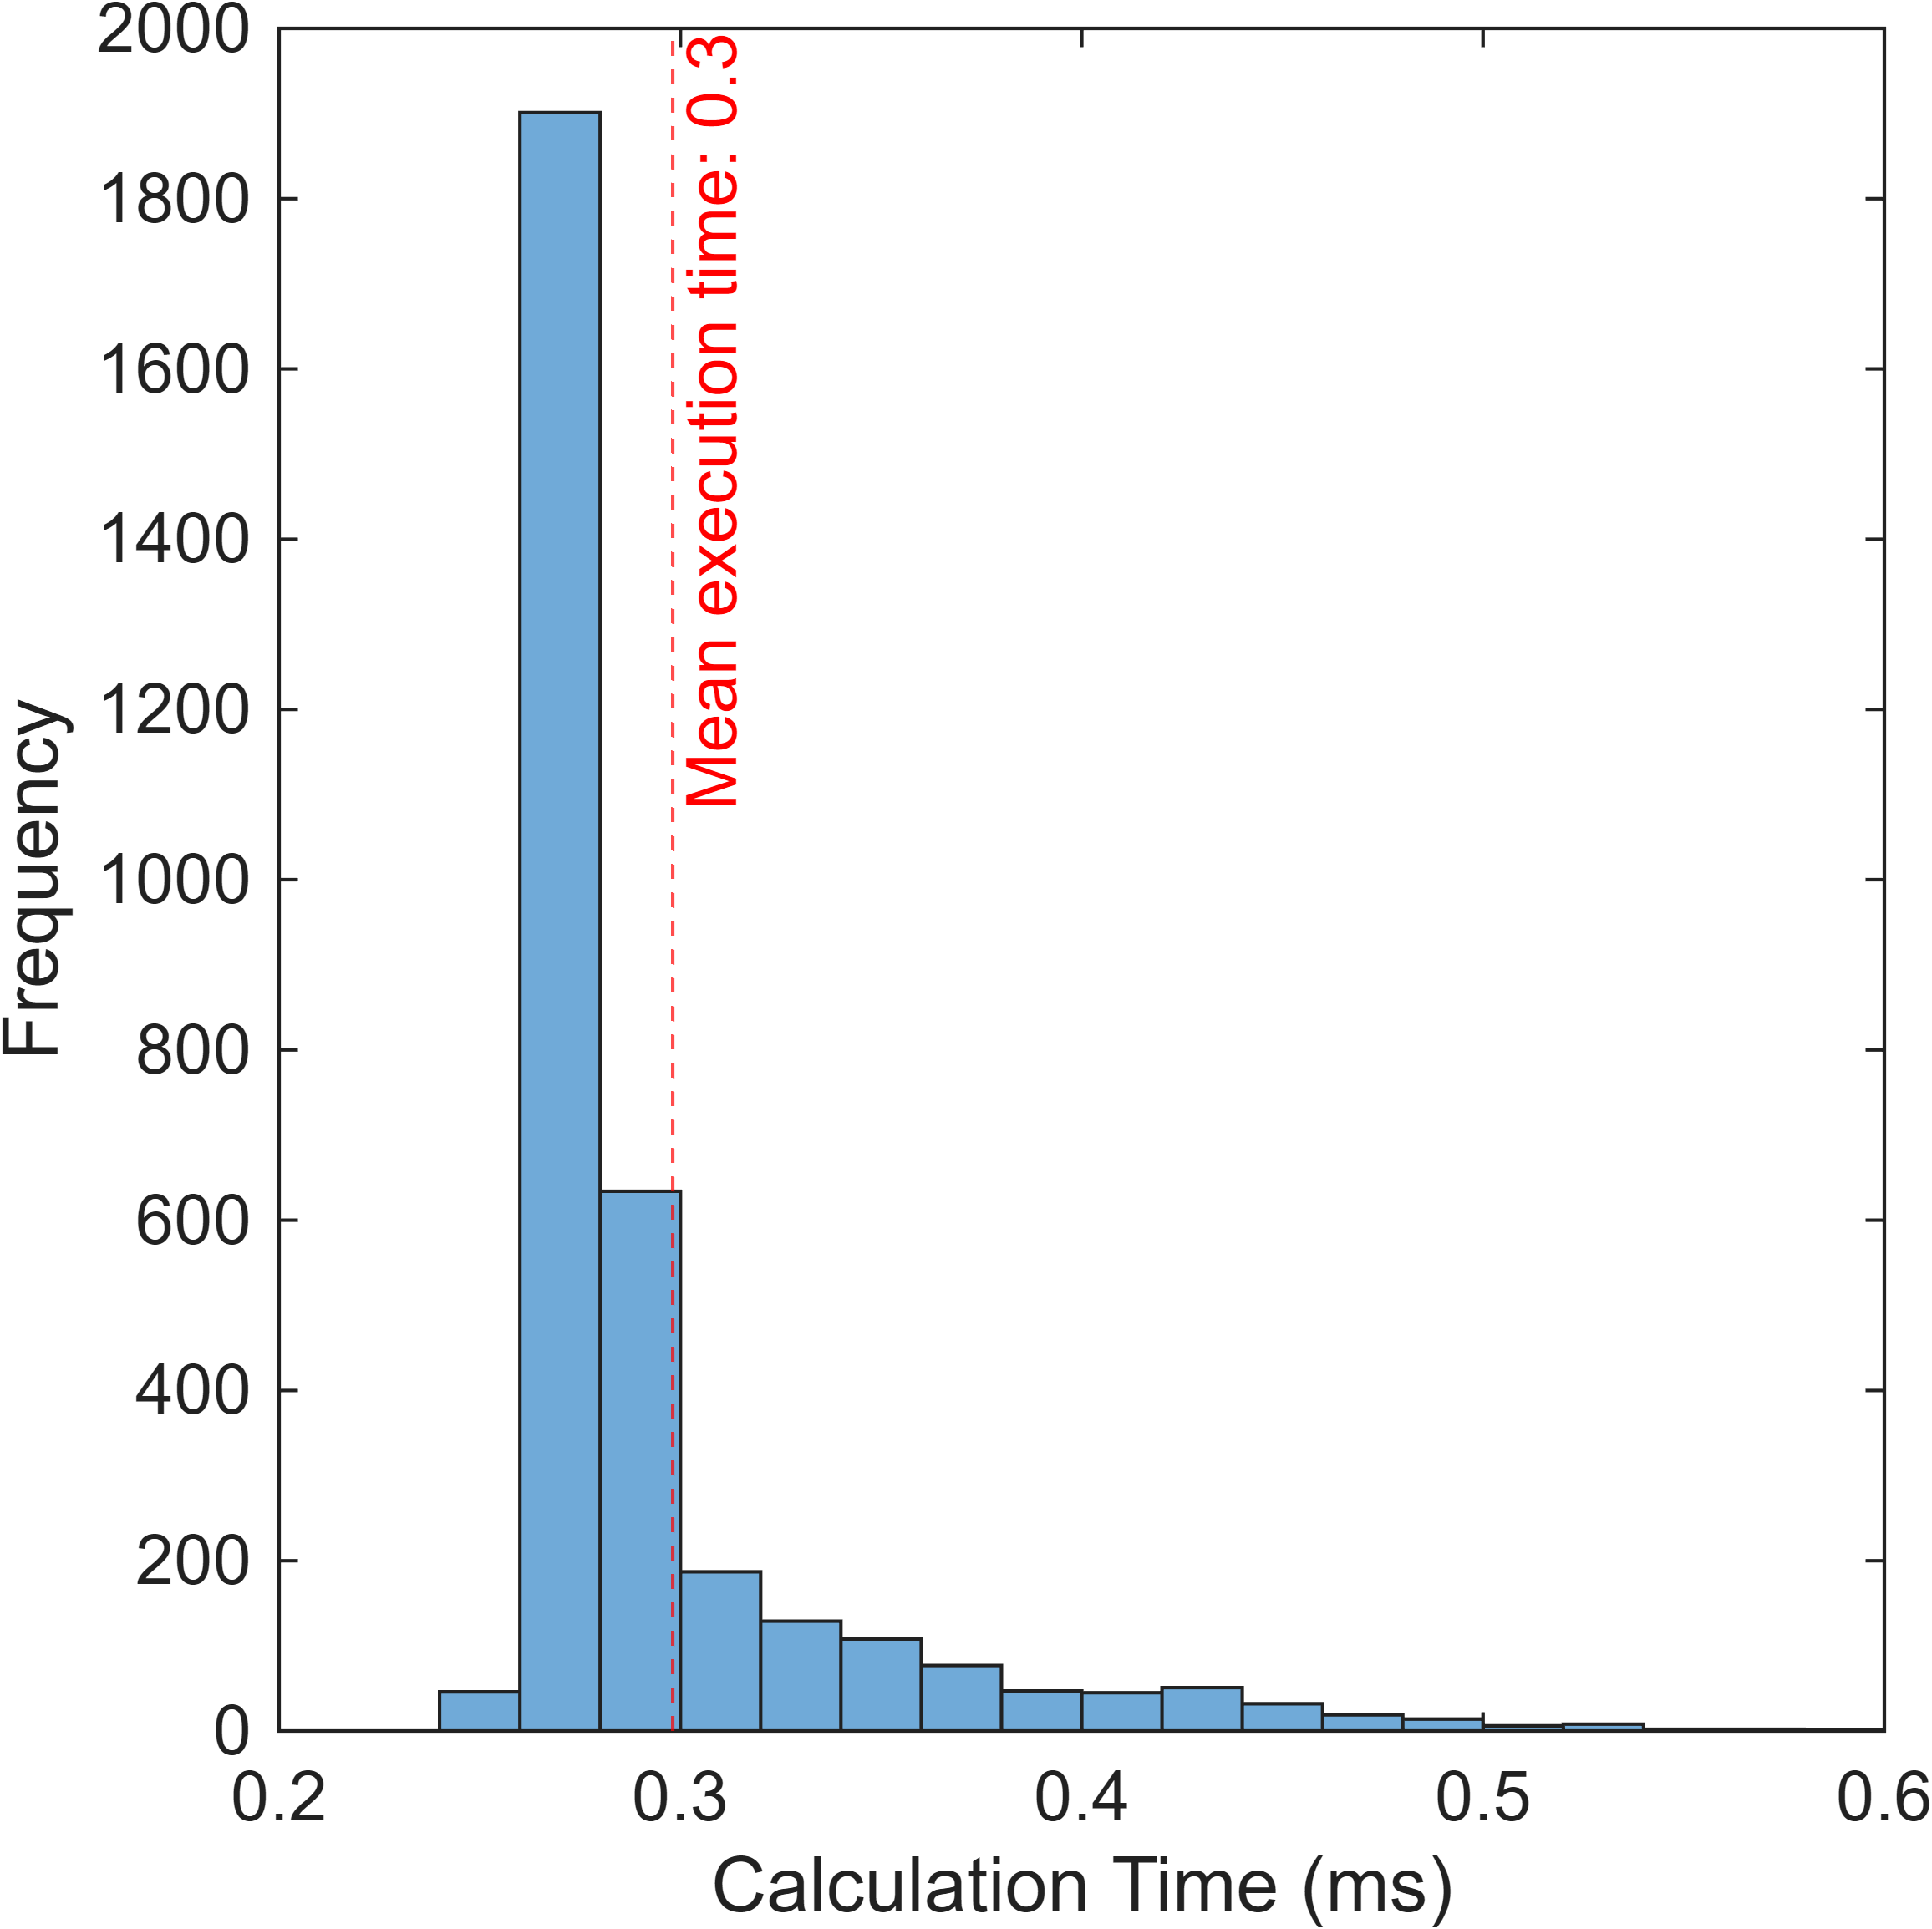
\includegraphics[scale=0.7]{figures/simulation-time.png}
\end{center}
\caption{Distribution of $n = 3325$ execution times for one arc trajectory, with mean execution time of 0.3 ms for the EKF}
\label{fig:ekf-exec-time}
\end{figure}

Given the simplicity of the EKF, the mean execution time of 0.3ms is well within the requirement of 10ms imposed by the sampling period. 

